% Options for packages loaded elsewhere
\PassOptionsToPackage{unicode}{hyperref}
\PassOptionsToPackage{hyphens}{url}
\PassOptionsToPackage{dvipsnames,svgnames,x11names}{xcolor}
%
\documentclass[
  a4paper,
]{article}

\usepackage{amsmath,amssymb}
\usepackage{iftex}
\ifPDFTeX
  \usepackage[T1]{fontenc}
  \usepackage[utf8]{inputenc}
  \usepackage{textcomp} % provide euro and other symbols
\else % if luatex or xetex
  \usepackage{unicode-math}
  \defaultfontfeatures{Scale=MatchLowercase}
  \defaultfontfeatures[\rmfamily]{Ligatures=TeX,Scale=1}
\fi
\usepackage{lmodern}
\ifPDFTeX\else  
    % xetex/luatex font selection
\fi
% Use upquote if available, for straight quotes in verbatim environments
\IfFileExists{upquote.sty}{\usepackage{upquote}}{}
\IfFileExists{microtype.sty}{% use microtype if available
  \usepackage[]{microtype}
  \UseMicrotypeSet[protrusion]{basicmath} % disable protrusion for tt fonts
}{}
\makeatletter
\@ifundefined{KOMAClassName}{% if non-KOMA class
  \IfFileExists{parskip.sty}{%
    \usepackage{parskip}
  }{% else
    \setlength{\parindent}{0pt}
    \setlength{\parskip}{6pt plus 2pt minus 1pt}}
}{% if KOMA class
  \KOMAoptions{parskip=half}}
\makeatother
\usepackage{xcolor}
\usepackage[paperwidth=8.00in,paperheight=10.00in,left=1.25in,textwidth=
5.25in,top=1.00in,textheight=8.25in]{geometry}
\setlength{\emergencystretch}{3em} % prevent overfull lines
\setcounter{secnumdepth}{5}
% Make \paragraph and \subparagraph free-standing
\ifx\paragraph\undefined\else
  \let\oldparagraph\paragraph
  \renewcommand{\paragraph}[1]{\oldparagraph{#1}\mbox{}}
\fi
\ifx\subparagraph\undefined\else
  \let\oldsubparagraph\subparagraph
  \renewcommand{\subparagraph}[1]{\oldsubparagraph{#1}\mbox{}}
\fi


\providecommand{\tightlist}{%
  \setlength{\itemsep}{0pt}\setlength{\parskip}{0pt}}\usepackage{longtable,booktabs,array}
\usepackage{calc} % for calculating minipage widths
% Correct order of tables after \paragraph or \subparagraph
\usepackage{etoolbox}
\makeatletter
\patchcmd\longtable{\par}{\if@noskipsec\mbox{}\fi\par}{}{}
\makeatother
% Allow footnotes in longtable head/foot
\IfFileExists{footnotehyper.sty}{\usepackage{footnotehyper}}{\usepackage{footnote}}
\makesavenoteenv{longtable}
\usepackage{graphicx}
\makeatletter
\def\maxwidth{\ifdim\Gin@nat@width>\linewidth\linewidth\else\Gin@nat@width\fi}
\def\maxheight{\ifdim\Gin@nat@height>\textheight\textheight\else\Gin@nat@height\fi}
\makeatother
% Scale images if necessary, so that they will not overflow the page
% margins by default, and it is still possible to overwrite the defaults
% using explicit options in \includegraphics[width, height, ...]{}
\setkeys{Gin}{width=\maxwidth,height=\maxheight,keepaspectratio}
% Set default figure placement to htbp
\makeatletter
\def\fps@figure{htbp}
\makeatother
% definitions for citeproc citations
\NewDocumentCommand\citeproctext{}{}
\NewDocumentCommand\citeproc{mm}{%
  \begingroup\def\citeproctext{#2}\cite{#1}\endgroup}
\makeatletter
 % allow citations to break across lines
 \let\@cite@ofmt\@firstofone
 % avoid brackets around text for \cite:
 \def\@biblabel#1{}
 \def\@cite#1#2{{#1\if@tempswa , #2\fi}}
\makeatother
\newlength{\cslhangindent}
\setlength{\cslhangindent}{1.5em}
\newlength{\csllabelwidth}
\setlength{\csllabelwidth}{3em}
\newenvironment{CSLReferences}[2] % #1 hanging-indent, #2 entry-spacing
 {\begin{list}{}{%
  \setlength{\itemindent}{0pt}
  \setlength{\leftmargin}{0pt}
  \setlength{\parsep}{0pt}
  % turn on hanging indent if param 1 is 1
  \ifodd #1
   \setlength{\leftmargin}{\cslhangindent}
   \setlength{\itemindent}{-1\cslhangindent}
  \fi
  % set entry spacing
  \setlength{\itemsep}{#2\baselineskip}}}
 {\end{list}}
\usepackage{calc}
\newcommand{\CSLBlock}[1]{\hfill\break\parbox[t]{\linewidth}{\strut\ignorespaces#1\strut}}
\newcommand{\CSLLeftMargin}[1]{\parbox[t]{\csllabelwidth}{\strut#1\strut}}
\newcommand{\CSLRightInline}[1]{\parbox[t]{\linewidth - \csllabelwidth}{\strut#1\strut}}
\newcommand{\CSLIndent}[1]{\hspace{\cslhangindent}#1}

\makeatletter
\@ifpackageloaded{tcolorbox}{}{\usepackage[skins,breakable]{tcolorbox}}
\@ifpackageloaded{fontawesome5}{}{\usepackage{fontawesome5}}
\definecolor{quarto-callout-color}{HTML}{909090}
\definecolor{quarto-callout-note-color}{HTML}{0758E5}
\definecolor{quarto-callout-important-color}{HTML}{CC1914}
\definecolor{quarto-callout-warning-color}{HTML}{EB9113}
\definecolor{quarto-callout-tip-color}{HTML}{00A047}
\definecolor{quarto-callout-caution-color}{HTML}{FC5300}
\definecolor{quarto-callout-color-frame}{HTML}{acacac}
\definecolor{quarto-callout-note-color-frame}{HTML}{4582ec}
\definecolor{quarto-callout-important-color-frame}{HTML}{d9534f}
\definecolor{quarto-callout-warning-color-frame}{HTML}{f0ad4e}
\definecolor{quarto-callout-tip-color-frame}{HTML}{02b875}
\definecolor{quarto-callout-caution-color-frame}{HTML}{fd7e14}
\makeatother
\makeatletter
\@ifpackageloaded{bookmark}{}{\usepackage{bookmark}}
\makeatother
\makeatletter
\@ifpackageloaded{caption}{}{\usepackage{caption}}
\AtBeginDocument{%
\ifdefined\contentsname
  \renewcommand*\contentsname{Table of contents}
\else
  \newcommand\contentsname{Table of contents}
\fi
\ifdefined\listfigurename
  \renewcommand*\listfigurename{List of Figures}
\else
  \newcommand\listfigurename{List of Figures}
\fi
\ifdefined\listtablename
  \renewcommand*\listtablename{List of Tables}
\else
  \newcommand\listtablename{List of Tables}
\fi
\ifdefined\figurename
  \renewcommand*\figurename{Figure}
\else
  \newcommand\figurename{Figure}
\fi
\ifdefined\tablename
  \renewcommand*\tablename{Table}
\else
  \newcommand\tablename{Table}
\fi
}
\@ifpackageloaded{float}{}{\usepackage{float}}
\floatstyle{ruled}
\@ifundefined{c@chapter}{\newfloat{codelisting}{h}{lop}}{\newfloat{codelisting}{h}{lop}[chapter]}
\floatname{codelisting}{Listing}
\newcommand*\listoflistings{\listof{codelisting}{List of Listings}}
\makeatother
\makeatletter
\makeatother
\makeatletter
\@ifpackageloaded{caption}{}{\usepackage{caption}}
\@ifpackageloaded{subcaption}{}{\usepackage{subcaption}}
\makeatother
\ifLuaTeX
  \usepackage{selnolig}  % disable illegal ligatures
\fi
\usepackage{bookmark}

\IfFileExists{xurl.sty}{\usepackage{xurl}}{} % add URL line breaks if available
\urlstyle{same} % disable monospaced font for URLs
\hypersetup{
  pdftitle={Artigo à Prova de Futuro},
  colorlinks=true,
  linkcolor={blue},
  filecolor={Maroon},
  citecolor={Blue},
  urlcolor={Blue},
  pdfcreator={LaTeX via pandoc}}

\title{Artigo à Prova de Futuro}
\usepackage{etoolbox}
\makeatletter
\providecommand{\subtitle}[1]{% add subtitle to \maketitle
  \apptocmd{\@title}{\par {\large #1 \par}}{}{}
}
\makeatother
\subtitle{Jornada de Open Science na Prática}
\author{}
\date{}

\begin{document}
\maketitle

\bookmarksetup{startatroot}

\section*{Home 🏢}\label{sec-home}

\markboth{Home 🏢}{Home 🏢}

Página do curso \textbf{``Artigo à Prova de Futuro: Jornada de Open
Science na Prática''}. Aqui você encontrará informações sobre o programa
do curso, materiais para seu acompanhamento e sugestões de leituras
sobre a prática da ciência aberta (artigos, notas de aulas, blogs,
vídeos, etc.).

Caso você caiu nessa página por acaso (🤣😁😉), saiba que o poderá se
inscrever no curso \href{https://forms.gle/b6Zio7oL8XxxhhtS9}{aqui}:
independente se ele estiver acontecendo no momento, será convidado a
participar da próxima versão.

\subsection*{Sobre os instrutores}\label{sec-instrutor}

\markright{Sobre os instrutores}

O curso é coordenado e ministrado por Pablo Rogers, doutor em
administração pela Universidade de São Paulo (FEA/USP) e professor de
finanças e métodos quantitativos desde 2005. Em sua
\href{https://github.com/phdpablo}{página de perfil do Github} temos
informações de seus trabalhos recentes, e no seu
\href{https://phdpablo.com/}{site pessoal}, detalhes sobre suas
formações, competências, trajetória e projetos.

Na sua versão atual o curso também será ministrado por Ricardo Limongi,
doutor em administração pela Fundação Getúlio Vargas (FGV-SP) e
professor de marketing e métodos quantitativos desde 2008 e atual editor
chefe da Brazilian Administration Review (BAR). Em seu
\href{https://www.instagram.com/limongi/}{perfil do Instagram} é
possível acompanhar sua agenda de atividades, cursos e palestras sobre
inteligência artificial aplicada aos negócios e pesquisa. Em seu
\href{https://www.youtube.com/@ricardolimongi_ia}{canal do YouTube}, é
possível encontrar vídeos das suas atividades: congressos, palestras,
aulas, etc.

\subsection*{Sobre o curso}\label{sec-about}

\markright{Sobre o curso}

O curso tem objetivo de introduzir os conceitos relacionados com a
ciência aberta e a prática da pesquisa reprodutível. O curso aborda
temas introdutórios sobre ciência aberta, com foco no ferramental
disponível para tornar a pesquisa mais transparente, reprodutível e
acessível. O curso é voltado para pesquisadores e estudantes de
pós-graduação, mas aberto a qualquer pessoa interessada em aprender
sobre a prática da ciência aberta. O protagonista do curso é o
pesquisador brasileiro que deseja aprimorar a qualidade e a
transparência de sua pesquisa, e que busca ferramentas para tornar-lá
mais eficiente e acessível.

Trata-se de um curso intermitente programado para acontecer em 4
encontros de 4 horas/aula (ou 8 encontros de 2 horas/aula), totalizando
16 horas/aula. Num primeiro momento, a ideia que o curso seja remoto e
síncrono para alcançar um número maior de interessados. Ele poderá
acontecer mais de uma vez no ano, com datas e horários a serem
definidos. Para o calendário atual do curso, consulte a seção
\href{https://phdpablo.github.io/curso-open-science/00-schedule.html}{Agenda}.

O curso é gratuito e com de certificado de extensão pela Universidade
Federal de Uberlândia (UFU). As inscrições são feitas por meio de um
\href{https://forms.gle/wRNWAU9Ffyp7o4Vq9}{formulário} intermediado pelo
projeto
\href{https://www.youtube.com/c/PsicoEconoMETRIA}{Psico\&Econo\_METRIA}.
Quando da previsão das datas, uma campanha de e-mail marketing divulgará
o link para a inscrição através de coordenações de pós-graduações
selecionadas.

As vagas são limitadas e a seleção será feita por ordem de inscrição.
Após o preenchimento das vagas, os demais interessados serão inscritos
automaticamente numa lista de espera e, tempestivamente, serão avisados
sobre a próxima edição do curso. Após selecionados, os inscritos
receberão um e-mail com instruções para acesso à plataforma de aulas
síncronas e para a realização das atividades prévias ao curso.

\subsection*{Ementa do curso}\label{sec-ementa}

\markright{Ementa do curso}

Introdução da Ciência Aberta / Repositórios da Ciência Aberta /
Gerenciamento de Referências e Bibliotecas / Gestão de Dados e Projetos
/ Controle de Versão / Documentos Reprodutíveis / Controle de Ambiente
(containers) / IA Aplicada à Pesquisa Científica.

\subsection*{Metodologia}\label{sec-method}

\markright{Metodologia}

Num primeiro momento, o curso foi concebido para acontecer de forma
remota e síncrona, com aulas expositivas e teóricas, porém em grande
medida, o conteúdo é essencialmente prático. Algumas aulas poderão ser
gravadas e disponibilizadas no
\href{https://www.youtube.com/c/PsicoEconoMETRIA}{canal do YouTube do
projeto Psico\&Econo\_METRIA}, mas a intenção é que o conteúdo principal
seja síncrono, para uma maior interação entre os participantes.

Nesse sentido, o material do curso organizado nessa página refere-se ao
roteiro estruturado de tudo que se vê nas aulas síncronas e conteúdos
adicionais (bibliografia, notas de aulas, links, etc).

Artigo à Prova de Futuro: Jornada de Open Science na Prática by Pablo
Rogers is licensed under CC BY-NC-SA 4.0

\bookmarksetup{startatroot}

\section*{Pré-requisitos 📇}\label{sec-prework}

\markboth{Pré-requisitos 📇}{Pré-requisitos 📇}

O curso não exige conhecimento prévio em programação, mas é recomendável
que o aluno tenha familiaridade com o uso de computadores (ambiente
Windows) e com a escrita de textos científicos. Nesse sentido, não é
necessário ter conhecimento prévio sobre as ferramentas e plataformas
que utilizaremos no curso: Zotero, OSF, Zenodo, Git, Github, RStudio,
Quarto/RMarkdown, Docker, etc; mas desejável que o aluno já as tenha
instalado e/ou cadastro nas plataformas.

Abaixo eu descrevo sucintamente o que é cada uma dessas ferramentas e
plataformas, e como você pode se preparar para o curso. Também apresento
um vídeo curto sobre a instalação e cadastro em cada uma delas. A ideia
é que você já tenha todas as ferramentas e plataformas instaladas e/ou
cadastro antes do início do curso, para que possamos focar no conteúdo e
prática durante as aulas síncronas. Mas pode ficar tranquilo, pois na
primeira aula do curso abordaremos essas tarefas, e caso ainda haja
alguma dúvida na instalação e cadastro, dedicaremos algum tempo para
saná-las.

Outras soluções que iremos discutir e testar durante o curso, como
alguns pacotes do R, e aplicações de IA no último módulo, deixaremos
para as aulas remotas. Essas soluções na sua maioria requerem cadastros
rápidos, e podem ser feitos de forma instantânea via conta
Google/Microsoft/Apple.

\begin{tcolorbox}[enhanced jigsaw, leftrule=.75mm, left=2mm, toprule=.15mm, opacitybacktitle=0.6, colback=white, titlerule=0mm, colbacktitle=quarto-callout-important-color!10!white, bottomtitle=1mm, bottomrule=.15mm, opacityback=0, rightrule=.15mm, toptitle=1mm, title=\textcolor{quarto-callout-important-color}{\faExclamation}\hspace{0.5em}{ChatGPT para suas notas de leituras}, colframe=quarto-callout-important-color-frame, arc=.35mm, breakable, coltitle=black]

Os resumos das bibliografias que apresento nas seções seguintes foram
elaborados com o auxílio do ChatGPT 4, seja pelo o
\href{https://chat.openai.com/}{webapp da OpenAI} ou pelo
\href{https://copilot.microsoft.com/}{Copilot} (ou buscador Bing) da
Microsoft.

Eu destaco (seleciono através de marca texto no Zotero, por exemplo) as
passagens que considero importante do artigo científico, tendo em vista
a minha perspectiva e fins no momento da leitura, e posteriormente copio
e colo as notas de leitura com a seguinte prompt:

``\emph{Senteces in the text are reading notes, that is, what I found
most important and interesting, from a scientific article on the topic
open science. I would like you to summarize the notes in a descriptive
text and concatenate the arguments highlighted in the notes. Give your
answer in Portuguese}''

\end{tcolorbox}

\begin{tcolorbox}[enhanced jigsaw, leftrule=.75mm, left=2mm, toprule=.15mm, opacitybacktitle=0.6, colback=white, titlerule=0mm, colbacktitle=quarto-callout-caution-color!10!white, bottomtitle=1mm, bottomrule=.15mm, opacityback=0, rightrule=.15mm, toptitle=1mm, title=\textcolor{quarto-callout-caution-color}{\faFire}\hspace{0.5em}{Não confie cegamente na IA}, colframe=quarto-callout-caution-color-frame, arc=.35mm, breakable, coltitle=black]

Eu simplesmente copiei e colei os resultados do ChatGPT para compilar
essas notas de leituras? Não. Após o resultado do ChatGPT eu reviso o
sumário das notas de leituras e faço ajustes, que somente são possíveis
porque li o artigo por completo. A despeito do ChatGPT fazer um bom
serviço nesse sentido, ele ainda comete muitos deslizes. Deslizes esses
que você não pode deixar passar num texto científico, e somente captaria
a partir da leitura do artigo ou sendo conhecedor do assunto abordado.

\end{tcolorbox}

\begin{tcolorbox}[enhanced jigsaw, leftrule=.75mm, left=2mm, toprule=.15mm, opacitybacktitle=0.6, colback=white, titlerule=0mm, colbacktitle=quarto-callout-note-color!10!white, bottomtitle=1mm, bottomrule=.15mm, opacityback=0, rightrule=.15mm, toptitle=1mm, title=\textcolor{quarto-callout-note-color}{\faInfo}\hspace{0.5em}{Outra curiosidade\ldots{}}, colframe=quarto-callout-note-color-frame, arc=.35mm, breakable, coltitle=black]

A
\href{https://phdpablo.github.io/curso-open-science/img/cover.png}{imagem
cover desse curso} foi gerada por uma IA, com posteriores ajustes (off
course!). Existem diversos geradores de imagens que você pode testar
gratuitamente, mas eu costumo utilizar o i)
\href{https://openai.com/dall-e/}{DALL-E}, que é uma solução da OpenAI
que também pode ser utilizada no
\href{https://copilot.microsoft.com/}{Copilot da Microsoft}; ii) o
\href{https://playgroundai.com/}{PlaygroundAI}, e iii) o
\href{https://gemini.google.com/app}{Gemini} do Google.

\end{tcolorbox}

\subsection*{Github}\label{sec-githubprework}
\addcontentsline{toc}{subsection}{Github}

\markright{Github}

Primeiramente, se cadastre no Github: \url{https://github.com/signup},
pois com ele você poderá acessar o material do curso e interagir com os
demais participantes. E com a conta do Github você também poderá se
cadastrar em outras plataformas, como o Zenodo, OSF, etc. Algumas
features que aprenderemos no curso exigem o vínculo entre as contas. Se
for professor ou estudante, você pode solicitar o
\href{https://education.github.com/}{GitHub Education} e ter acesso, por
exemplo, ao Copilot, uma das ferramentas de IA que abordaremos no último
módulo. Por isso, é importante que você se cadastre com um e-mail
institucional. Use o mesmo e-mail para se cadastrar em todas
plataformas.

\url{https://youtu.be/Nmjh9KsV6eU}

\subsection*{Git}\label{sec-gitprework}
\addcontentsline{toc}{subsection}{Git}

\markright{Git}

Github não é a mesma coisa que Git. O Github é uma plataforma, e o Git é
uma ferramenta. Instale a versão mais recente do Git:
\url{https://git-scm.com/downloads}. O Git é uma ferramenta de controle
de versão, e o Github é uma plataforma que utiliza o Git. O Git é uma
ferramenta essencial para a prática da ciência aberta, e é uma das
ferramentas mais importantes para o pesquisador que deseja tornar sua
pesquisa mais transparente e reprodutível.

\url{https://youtu.be/XCa6mE0bEI0}

\subsection*{Zotero}\label{sec-zoteroprework}
\addcontentsline{toc}{subsection}{Zotero}

\markright{Zotero}

Baixe a versão mais recente do Zotero:
\url{https://www.zotero.org/download/} e cadastre uma conta:
\url{https://www.zotero.org/user/register/}. Vamos discutir sobre o
Zotero e diversos plugins que são úteis no dia-a-dia do pesquisador.
Atualmente, o Zotero é a ferramenta mais completa para gerenciamento de
referências e bibliotecas, e se integra nativamente com o RStudio.

\url{https://youtu.be/ZSFq6LHaDJ4}

\subsection*{OSF}\label{sec-osfprework}
\addcontentsline{toc}{subsection}{OSF}

\markright{OSF}

Cadastre no Open Science Framework (OSF):
\url{https://osf.io/register/}. Como veremos, essa plataforma é uma das
mais importantes para a prática da ciência aberta. Ela está no começo
(pré-registro) e no final (repositório de dados e pré-print) do ciclo de
vida (workflow) de um projeto de pesquisa.

\url{https://youtu.be/WQ4O-8O6MwI}

\subsection*{Zenodo}\label{sec-zenodoprework}
\addcontentsline{toc}{subsection}{Zenodo}

\markright{Zenodo}

Apesar do Zenodo cumprir funções similares ao OSF e até mesmo ao Github,
ele é mais voltado para a publicação de dados e publicações científicas.
Cadastre no Zenodo: \url{https://zenodo.org/login/} e víncule sua conta
com o Github. Isso será útil, principalmente, para geração de DOI de
repositórios do Github.

\url{https://youtu.be/pZaqL3Auxb0}

\subsection*{RStudio}\label{sec-rstudioprework}
\addcontentsline{toc}{subsection}{RStudio}

\markright{RStudio}

Baixe a versão mais recente do RStudio:
\url{https://posit.co/download/rstudio-desktop/}. O RStudio é uma
Integrated Development Environment (IDE) para a linguagem R. O RStudio é
uma ferramenta essencial para a prática da ciência aberta em R, pois
integra as principais soluções que abordaremos no curso (Zotero, Quarto,
Git/Github, etc.). A empresa RStudio recentemente mudou o nome para
Posit, com o objetivo refletir melhor a expansão da empresa para além do
desenvolvimento de ferramentas para R, incluindo Python e outras
linguagens. Nesse mesmo link você pode baixar o R, que é a linguagem de
programação que utilizaremos no curso.

\url{https://youtu.be/KM2jxaNIEUk}

\subsection*{Quarto}\label{sec-quartoprework}
\addcontentsline{toc}{subsection}{Quarto}

\markright{Quarto}

Baixe a versão mais recente do Quarto: \url{https://www.quarto.org/}. O
Quarto é uma linguagem de marcação que permite a criação de documentos
reprodutíveis e dinâmicos. Ele é uma evolução e tende a substituir o
RMarkdown, que é a principal linguagem de marcação do R. O Quarto
engloba e adiciona diversas outras vantagens ao RMarkdown, tal como a
possibilidade de criar documentos reprodutíveis em Python, Julia, etc.
Se você já tem algum conhecimento de RMarkdown, não se preocupe, pois o
Quarto é uma extensão natural.

\url{https://youtu.be/-HvOMVkk6I4}

\subsection*{Docker}\label{sec-dockerprework}
\addcontentsline{toc}{subsection}{Docker}

\markright{Docker}

Baixe a versão mais recente do Docker:
\url{https://www.docker.com/products/docker-desktop}. Nesse mesmo link
você cria uma conta. O Docker é uma plataforma para desenvolvimento,
envio e execução de aplicativos. O Docker é uma ferramenta essencial
para a prática da ciência aberta, pois permite a criação de ambientes
reprodutíveis.

\url{https://youtu.be/WjXQxhTLlrQ}

\bookmarksetup{startatroot}

\section*{Agenda 📅}\label{sec-schedule}

\markboth{Agenda 📅}{Agenda 📅}

Planejamento dos dias (📅) e horários das aulas (⏲️), conforme a ementa
do curso. Na seção de cada uma das aulas temos materiais adicionais para
o respectivo conteúdo. Quando disponível, por aqui, poderás acessar os
slides utilizados nas aulas (🗣️), aulas gravadas ou indicações de vídeo
(🎥) e leituras básica sobre os conteúdos (📓).

\begin{longtable}[]{@{}
  >{\raggedright\arraybackslash}p{(\columnwidth - 6\tabcolsep) * \real{0.2113}}
  >{\centering\arraybackslash}p{(\columnwidth - 6\tabcolsep) * \real{0.2676}}
  >{\centering\arraybackslash}p{(\columnwidth - 6\tabcolsep) * \real{0.2817}}
  >{\centering\arraybackslash}p{(\columnwidth - 6\tabcolsep) * \real{0.2394}}@{}}
\toprule\noalign{}
\begin{minipage}[b]{\linewidth}\raggedright
Aula/Conteúdo
\end{minipage} & \begin{minipage}[b]{\linewidth}\centering
Data
\end{minipage} & \begin{minipage}[b]{\linewidth}\centering
Material Principal
\end{minipage} & \begin{minipage}[b]{\linewidth}\centering
Instrutor
\end{minipage} \\
\midrule\noalign{}
\endhead
\bottomrule\noalign{}
\endlastfoot
Chapter~\ref{sec-intro} & 📅04/06/24⏲️19:00 & 🗣️🎥📓 & Ricardo
Limongi \\
Chapter~\ref{sec-osf} & 📅06/06/24⏲️19:00 & 🗣️🎥📓 & Pablo Rogers \\
Chapter~\ref{sec-zotero} & 📅11/06/24⏲️19:00 & 🗣️🎥📓 & Pablo Rogers \\
Chapter~\ref{sec-project} & 📅13/06/24⏲️19:00 & 🗣️🎥📓 & Pablo Rogers \\
Chapter~\ref{sec-git} & 📅18/06/24⏲️19:00 & 🗣️🎥📓 & Pablo Rogers \\
Chapter~\ref{sec-quarto} & 📅20/06/24⏲️19:00 & 🗣️🎥📓 & Pablo Rogers \\
Chapter~\ref{sec-docker} & 📅25/06/24⏲️19:00 & 🗣️🎥📓 & Pablo Rogers \\
Chapter~\ref{sec-AI} & 📅27/06/24⏲️19:00 & 🗣️🎥📓 & Ricardo Limongi \\
\end{longtable}

\bookmarksetup{startatroot}

\section{Introdução à Ciência Aberta}\label{sec-intro}

\bookmarksetup{startatroot}

\section{Repositórios da Ciência Aberta}\label{sec-osf}

No contexto da ciência aberta, existem diversos repositórios
disponíveis, cada um com suas funções e propósitos específicos. Esses
repositórios são essenciais para promover a transparência,
acessibilidade e colaboração na pesquisa científica. Eles assumem um
papel crucial na democratização do conhecimento e na promoção da
colaboração científica. Cada qual com suas particularidades, oferecem
aos pesquisadores ferramentas para armazenar, compartilhar e gerenciar
dados, publicações e outros materiais de pesquisa, ou se preferir, todo
o ciclo de vida da pesquisa.

\begin{itemize}
\tightlist
\item
  \href{www.zenodo.org}{\textbf{Zenodo}}: é um repositório gerido pelo
  CERN em colaboração com o projeto
  \href{https://www.openaire.eu/}{OpenAIRE} da União Europeia. Oferece
  armazenamento gratuito e seguro para dados de pesquisa, com a
  capacidade de gerar DOIs para facilitar a citação dos dados.
\item
  \href{www.figshare.com}{\textbf{Figshare}}: é um repositório comercial
  que permite aos pesquisadores armazenar, compartilhar e descobrir
  dados de pesquisa. Oferece ferramentas para visualização de
  documentos, gráficos e outros tipos de dados diretamente no navegador,
  além de gerar DOIs para os projetos.
\item
  \href{data.mendeley.com}{\textbf{Mendeley Data}}: é um repositório de
  dados de pesquisa da Elsevier, permitindo o armazenamento,
  compartilhamento e citação de conjuntos de dados. Ele suporta uma
  ampla gama de tipos de dados e está integrado com a plataforma de
  referência Mendeley.
\item
  \href{dataverse.harvard.edu}{\textbf{Harvard Dataverse}}: é uma rede
  de repositórios que permite aos pesquisadores compartilhar, armazenar
  e citar dados de pesquisa. Ele oferece ferramentas avançadas para a
  gestão de dados, incluindo controle de versões e metadados ricos,
  essenciais para o gerenciamento do ciclo de vida da pesquisa.
\item
  \href{arxiv.org}{\textbf{arXiv}}: é um repositório de pré-impressões
  de artigos científicos em física, matemática, ciência da computação e
  outras áreas. Ele permite aos pesquisadores compartilhar seus
  trabalhos antes da revisão por pares, facilitando o acesso à pesquisa
  em estágios iniciais.
\item
  \href{github.com}{\textbf{Github}}: é uma plataforma de
  desenvolvimento colaborativo baseada em Git, amplamente utilizada por
  pesquisadores para compartilhar código, documentos e outros materiais
  de pesquisa. Ele oferece controle de versões, rastreamento de
  problemas e integração com outras ferramentas de desenvolvimento.
\end{itemize}

Além desses exemplos, poderíamos citar outras soluções que cumprem
papeis semelhantes ou focado em certas disciplinas:
\href{databrary.org}{Databrary}, \href{dataverse.no}{DataverseNO},
\href{dataone.org}{DataONE}, \href{datacite.org}{DataCite},
\href{datahub.io}{DataHub}, \href{datamed.org}{DataMed},
\href{datashare.is.ed.ac.uk}{DataShare},
\href{dataverse.org}{DataVerse}, \href{datadryad.org}{Dryad},
\href{earthchem.org}{EarthChem}, \href{eudat.eu}{EUDAT},
\href{www.ebi.ac.uk/ena/browser/home}{European Nucleotide Archive
(ENA)}, \href{ncbi.nlm.nih.gov/genbank}{GenBank},
\href{datasetsearch.research.google.com}{Google Dataset Search},
\href{hathitrust.org}{HathiTrust Research Center},
\href{icpsr.umich.edu}{ICPSR}, \href{jstor.org}{JSTOR Data for
Research}, \href{ncbi.nlm.nih.gov}{National Center for Biotechnology
Information (NCBI)}, \href{nih.gov}{National Institutes of Health (NIH)
Data Sharing Repositories}, \href{data.noaa.gov}{National Oceanographic
Data Center (NODC)}, \href{plos.org}{PLOS ONE},
\href{ncbi.nlm.nih.gov/pmc}{PubMed Central},
\href{researchdata.ands.org.au}{Research Data Australia} e
\href{ukdataservice.ac.uk}{UK Data Service}; e em última instância, as
redes sociais acadêmicas como \href{academia.edu}{Academia.edu},
\href{scholar.google.com}{Google Scholar}, \href{orcid.org}{ORCID} e
\href{researchgate.net}{ResearchGate}, também podem ser usadas para
compartilhar e descobrir pesquisas.

A despeito de todas essas opções, vamos focar na plataforma
\href{https://osf.io/}{\textbf{Open Science Framework (OSF)}} para a
realização do nosso curso. O \textbf{OSF} é uma plataforma de código
aberto para colaboração em pesquisa, que oferece uma estrutura para
conectar os fluxos de trabalho de pesquisa, desde a concepção do projeto
até a publicação. O \textbf{OSF} é mantido pelo
\href{https://www.cos.io/}{Center for Open Science (COS)}, uma
organização sem fins lucrativos com sede nos Estados Unidos. O
\textbf{OSF} é um dos principais produtos do COS e é usado por
pesquisadores de todo o mundo para colaborar em projetos de pesquisa.

O \textbf{OSF} oferece uma série de recursos para ajudar os
pesquisadores a gerenciar seus projetos de pesquisa, incluindo:

\begin{itemize}
\tightlist
\item
  \textbf{Criar projetos de pesquisa}: organizar seus estudos, incluindo
  metadados, datasets, materiais de pesquisa e publicações.
\item
  \textbf{Carregar e publicar dados}: armazenar e compartilhar seus
  dados de forma segura e acessível.
\item
  \textbf{Colaboração em equipe}: convidar colaboradores para participar
  do projeto, atribuir tarefas e acompanhar o progresso.
\item
  \textbf{Integração com outras ferramentas}: conectar a armazenamentos
  nas nuvens (Box, DropBox, Google Drive e OneDrive), gerenciadores de
  referências (Zotero e Mendeley) e outros repositórios (Dataverse,
  Github, figsahre, etc).
\end{itemize}

O \textbf{OSF} tem um foco mais amplo em todo o ciclo de vida da
pesquisa, desde a concepção da ideia até a publicação dos resultados. Já
algumas das soluções citadas foca principalmente no compartilhamento de
dados e publicações. O \textbf{OSF} oferece ferramentas mais robustas
para colaboração em equipe, como wikis, painéis de discussão e
ferramentas de gerenciamento de tarefas, e principalmente, possui uma
comunidade mais ativa de pesquisadores e colaboradores.

\begin{center}
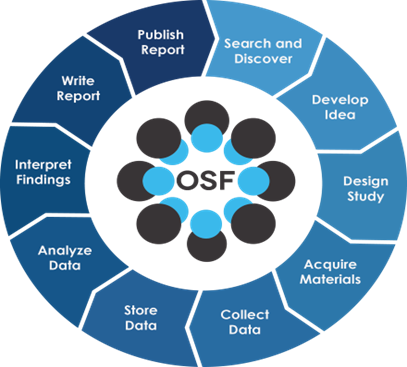
\includegraphics{img/osf-researchcycle.png}
\end{center}

\subsection{Open Science Framework
(OSF)}\label{open-science-framework-osf}

O material utilizado nesse módulo do curso segue de perto a proposta de
Olson et al. (2022), um \href{https://osf.io/yaqe8/}{projeto oficial do
COS} que possui recursos, modelos e práticas para ajudar os
pesquisadores a iniciar sua jornada \textbf{OSF}. Claro que ele foi
adaptado para nossos fins, principalmente, em decorrência do tempo
destinado ao módulo.

\begin{tcolorbox}[enhanced jigsaw, leftrule=.75mm, left=2mm, toprule=.15mm, opacitybacktitle=0.6, colback=white, titlerule=0mm, colbacktitle=quarto-callout-tip-color!10!white, bottomtitle=1mm, bottomrule=.15mm, opacityback=0, rightrule=.15mm, toptitle=1mm, title=\textcolor{quarto-callout-tip-color}{\faLightbulb}\hspace{0.5em}{Bifurcando ou duplicando um projeto}, colframe=quarto-callout-tip-color-frame, arc=.35mm, breakable, coltitle=black]

Você sabia que é possível executar um ``\emph{forking}'' (criar uma
cópia do projeto existente) ou ``\emph{duplicate as template}''
(duplicar apenas a estrutura do projeto e seus componentes) de um
projeto público no OSF?

Você que se interessa em iniciar seu próprio projeto OSF com um modelo,
pode criar sua própria duplicata do projeto Olson et al. (2022) para
começar!

Neste \href{https://osf.io/yaqe8/}{projeto}, existem templates e
recursos básicos para diversos casos de uso encontrados no OSF;
coordenação de equipes de pesquisa, planejamento de gerenciamento de
dados, documentos reprodutíveis e até mesmo gerenciamento de cursos.

\end{tcolorbox}

Para os alunos que desejam uma leitura sobre o \textbf{OSF} na prática,
indico os artigos de Sullivan, DeHaven, and Mellor (2019) e Soderberg
(2018). Apesar de o leitor poder encontrar \emph{prints} das telas da
plataforma desatualizadas, esses dois artigos podem ser um bom começo
para entender a lógica da plataforma. E \emph{off course}, recomendo
fortemente você dar uma olhada no
\href{https://help.osf.io/article/342-getting-started-on-the-osf}{suporte
do \textbf{OSF}}, onde podemos encontrar vídeos introdutórios
excelentes.

Esse curso poderia ter sido concebido e gerenciado dentro do
\textbf{OSF}, no entanto, devido a proposta de apresentarmos também o
\href{https://phdpablo.github.io/curso-open-science/05-git.html}{Git/Github}
e sua integração com documentos reprodutíveis no
\href{https://phdpablo.github.io/curso-open-science/06-quarto.html}{RStudio/Quarto}
(como esse que está lendo 😁), optamos por priorizar o repositório do
Github. Por isso, que também nesse módulo passamos pelo
\href{https://phdpablo.github.io/curso-open-science/00-prework.html\#sec-zenodoprework}{Zenodo},
que integra com o Github e tem a capacidade de gerar DOIs para as
versões dos repositórios.

\begin{tcolorbox}[enhanced jigsaw, leftrule=.75mm, left=2mm, toprule=.15mm, opacitybacktitle=0.6, colback=white, titlerule=0mm, colbacktitle=quarto-callout-note-color!10!white, bottomtitle=1mm, bottomrule=.15mm, opacityback=0, rightrule=.15mm, toptitle=1mm, title=\textcolor{quarto-callout-note-color}{\faInfo}\hspace{0.5em}{@sullivan2019 \emph{Reading Note}}, colframe=quarto-callout-note-color-frame, arc=.35mm, breakable, coltitle=black]

O artigo apresenta um protocolo para a implementação de práticas de
Ciência Aberta (CA), com foco no uso do Open Science Framework (OSF). As
principais ideias do texto são as seguintes:

\begin{itemize}
\item
  A CA é um movimento que promove a transparência, a reprodutibilidade e
  a acessibilidade dos resultados de pesquisa;
\item
  As práticas de CA podem contribuir para a melhoria da qualidade da
  pesquisa científica, tornando-a mais confiável e robusta;
\item
  O OSF é uma plataforma gratuita e de código aberto que pode ser usada
  para implementar práticas de CA;
\end{itemize}

O protocolo apresentado no texto fornece instruções passo a passo para
as seguintes práticas de CA:

\begin{itemize}
\item
  \textbf{Planejamento de gerenciamento de dados}: O planejamento de
  gerenciamento de dados é essencial para garantir que os dados de
  pesquisa sejam armazenados, organizados e gerenciados de forma
  eficiente e eficaz. O OSF fornece ferramentas para ajudar os
  pesquisadores a planejar e implementar seus planos de gerenciamento de
  dados.
\item
  \textbf{Pré-registro de estudos}: O pré-registro de estudos é uma
  prática que consiste em publicar um plano de pesquisa antes de iniciar
  o estudo. Isso ajuda a garantir que o estudo seja realizado de forma
  objetiva e transparente. O OSF fornece um recurso para pré-registrar
  estudos.
\item
  \textbf{Controle de versão}: O controle de versão é uma prática que
  consiste em rastrear as alterações feitas em arquivos de texto. Isso
  ajuda a garantir que os resultados de pesquisa sejam reprodutíveis e
  que as alterações feitas nos dados sejam rastreáveis. O OSF fornece
  ferramentas para gerenciar o controle de versão de arquivos de
  pesquisa.
\item
  \textbf{Compartilhamento de dados e materias}: O compartilhamento de
  dados e materiais de pesquisa é uma prática importante para aumentar a
  transparência e a reprodutibilidade da pesquisa. O OSF fornece um
  repositório para compartilhar dados e materiais de pesquisa.
\item
  \textbf{Publicação de pré-impressões}: As pré-impressões são versões
  preliminares de artigos científicos que são publicadas online antes de
  serem revisados por pares. As pré-impressões podem ajudar a acelerar a
  divulgação da pesquisa e a promover o debate científico. O OSF fornece
  um repositório para publicar pré-impressões.
\end{itemize}

O artigo fornece informações valiosas para os pesquisadores que desejam
implementar práticas de CA. O protocolo apresentado pode ser usado como
um guia para implementar essas práticas de forma eficaz.

\end{tcolorbox}

\bookmarksetup{startatroot}

\section{Gerenciamento de Referências e Bibliotecas}\label{sec-zotero}

\bookmarksetup{startatroot}

\section{Gestão de Dados e Projetos}\label{sec-project}

\bookmarksetup{startatroot}

\section{Controle de versão}\label{sec-git}

\bookmarksetup{startatroot}

\section{Documentos Reprodutíveis}\label{sec-quarto}

\bookmarksetup{startatroot}

\section{Controle de Ambiente (Containers)}\label{sec-docker}

\bookmarksetup{startatroot}

\section{IA Aplicada à Pesquisa Científica}\label{sec-AI}

\bookmarksetup{startatroot}

\section*{Referências}\label{referuxeancias}
\addcontentsline{toc}{section}{Referências}

\markboth{Referências}{Referências}

\phantomsection\label{refs}
\begin{CSLReferences}{1}{0}
\bibitem[\citeproctext]{ref-olson2022}
Olson, Eric, Nicole Pfeiffer, Mark Call, and Daniel Steger. 2022.
{``Getting Started on OSF,''} August.
\url{https://doi.org/10.17605/OSF.IO/YAQE8}.

\bibitem[\citeproctext]{ref-soderberg2018}
Soderberg, Courtney K. 2018. {``Using OSF to Share Data: A Step-by-Step
Guide.''} \emph{Advances in Methods and Practices in Psychological
Science} 1 (1): 115--20. \url{https://doi.org/10.1177/2515245918757689}.

\bibitem[\citeproctext]{ref-sullivan2019}
Sullivan, Ian, Alexander DeHaven, and David Mellor. 2019. {``Open and
Reproducible Research on Open Science Framework.''} \emph{Current
Protocols Essential Laboratory Techniques} 18 (1): e32.
\url{https://doi.org/10.1002/cpet.32}.

\end{CSLReferences}



\end{document}
